\documentclass[10pt]{article}

\usepackage[font=footnotesize,labelfont=bf]{caption}
\usepackage[margin=0.3in]{geometry}
\usepackage{graphicx}
\usepackage{listings}
\usepackage{setspace}
\usepackage{textcomp}
\usepackage{titling}
\usepackage{url}
\usepackage{xcolor}

\setlength{\parindent}{0em}
\setlength{\righthyphenmin}{62}

\definecolor{lightblue}{RGB}{0,130,186}
\definecolor{darkgreen}{RGB}{0,114,0}
\definecolor{darkpurple}{RGB}{125,0,183}

\lstset{
	language=Python,
	tabsize=4,
	basicstyle=\color{black}\footnotesize\ttfamily,
	keywordstyle=\color{black}\footnotesize\ttfamily, % style for keywords
	identifierstyle=\color{black}\footnotesize\ttfamily,
	commentstyle=\color{black}\footnotesize\ttfamily,
	numbers=left, % where to put the line-numbers
	numberstyle=\footnotesize\ttfamily, % the size of the fonts that are used for the line-numbers
	showstringspaces=false,
	breaklines=true
}

\begin{document}

\begin{singlespace}
	
	\begin{center}
		\begin{huge}
			Machine Learning Group Project Report
		\end{huge}
	\end{center}
	\bigskip
	
	\textbf{Team:} Abraham Ayooluwa Odukoya (16321320) / Sharon Olorunniwo (16323766) / Jack Harley (16317123)
	
	\bigskip
	
	\textbf{December 2020}\\
	\textbf{GitHub Project:} \url{https://github.com/JackHarley/Abyssalearn}
\end{singlespace}

\setlength{\parskip}{0.7em}

\section{Introduction}
	EVE Online is a space-based massively multiplayer online role playing game (MMORPG). Players participate in a large number of in-game activities including combat, trading, mining, manufacturing, exploration. The full extent of the game is beyond the scope of this project. The game is frequently featured in major media and news and has set numerous Guinness World Records.
	
	In EVE, all players pilot spaceships. They have to put "modules" on these ships which give it various statistics and abilities in combat. Modules come in various tiers called "meta levels", the lowest meta levels have the lowest statistics and are the cheapest, the higher meta levels have better statistics but are rarer and thus demand a higher price.
	
	As an example, there is a module in the game called a Stasis Webifier. This module is activated on a target ship and causes a reduction in their maximum velocity. It is essentially a way to hold a ship down so that it can be destroyed easier. Webifiers have a number of statistics including: range, percentage speed reduction and CPU usage.
	
	Players can combine a module with an item called a "mutaplasmid" to randomly change some statistics on the module, thus generating a new "mutated module" with unique statistics. For example, one random roll might increase range but decrease speed reduction and worsen its CPU usage. Players then sell these mutated modules on the contract market at a price of their choosing. Those who set a price too high will fail to see a sale, and those who set a price too low leave profit on the table. Our challenge is to produce a machine learning model which, given the statistics of a mutated module, can predict the best price it would sell for on the contracts market.
	
\section{Dataset and Features}
	EVE Online provides a JSON API conforming to the OpenAPI specification at https://esi.evetech.net/. Mutated modules or "abyssal modules" are traded using the in-game contracts system. A player lists an abyssal module with a specified price and players can browse contracts and search for modules that interest them. Only contracts that are currently actively listed are available from the API. Once they are sold, or if the owner delists them, they no longer show in the API.
	
	We implemented a data scraping solution which is implemented in the code file \textbf{scrape.py}. Data is stored in a SQLite database stored at \textbf{data/database.db}. The schema for this database is defined in \textbf{database.db} and consists of 4 tables. 
	
	Upon calling the scrape function, the system downloads all of the contracts currently listed in the API and stores their details in the database. It searches through each contract looking for abyssal modules. When an abyssal module is discovered, its details are downloaded and also stored. The details stored include the full raw "dogma attribute" information provided by the EVE servers, which are the numbers that define how powerful the module is in various ways. These dogma attribute values are our input features ($X$). The price of the contract is the output ($Y$). We deployed this code to a cloud server and created an automated task to run the scraping every 10 minutes, and left it to run for approximately one week to fill the database.
	
	Access to the scraped data is handled in code implemented in the access.py code file. The random\_item() function generates textual output of a random item of a specific type in the database. This was used for testing/debugging early on in the project and to validate that accurate data was being scraped. Here is an example of a stasis webifier item from the database, please note that some of the attributes have been cut out to reduce space taken in the report:
	
	\begin{lstlisting}
$ python main.py random 47702
Type: Abyssal Stasis Webifier
List Price: 12,000,000 ISK
Attributes:
Maximum Velocity Bonus        (#20):    -58.209600
CPU usage                     (#50):    31.494000
Optimal Range                 (#54):    11412.499762
	\end{lstlisting}

	The name of the item and price (output $Y$) is listed first. Then each of the dogma attributes (input features $X$) are listed with their name and value. The ID of the dogma attribute is listed in brackets and can be ignored, it is only for internal use. Certain attributes are blacklisted using a hardcoded list. These are attributes that are either known to never change or to be completely irrelevant to the price of the item. For example attribute ID 182 is blacklisted because this attribute simply gives the ID of the in-game skill required to use the item. This never changes between items of the same type and is not relevant to the price determination.
	
	The generate\_summary() function produces textual output showing each abyssal item, its type id and the number of data points currently available in the database. This was used to monitor the scraping progress of the program and choose items for our analysis once the data scraping was complete.
	
	The most important function is the item\_matrix() function. Our machine learning code calls this function with a type ID and it returns a 2D matrix (represented as a 2D Python list) of all the current data points for that type ID. The first column of the matrix is the price (output $Y$) of each item, and all subsequent columns are input features $X$. Here is an example of three rows of the matrix for the stasis webifier item:
	
	\begin{lstlisting}
$ python main.py matrix 47702
[350000000, 0.0, 9.9159999614954, 40.0, -58.42799962520599, 0.0, 5.0, 0.01, 25.285000208020207, 1.0, 5.0, 16296.000622510912, 30.0, 5000.0, 2115.0, 0.0, 0.0], 
[450000000, 0.0, 4.827999885678292, 40.0, -62.06400049209595, 0.0, 5.0, 0.01, 36.92250000983477, 1.0, 5.0, 16212.000615000727, 30.0, 5000.0, 2115.0, 0.0, 0.0], 
[1300000000, 0.0, 11.667999987602236, 40.0, -63.40800081253052, 0.0, 5.0, 0.01, 20.61250028759241, 1.0, 5.0, 15898.4005869627, 30.0, 5000.0, 2115.0, 0.0, 0.0]
	\end{lstlisting}

	This 2D list can then be fed into any machine learning model desired, with very little need for alteration.
		
	
\section{Methods}
	\subsection{Linear Regression}
		Linear regression is used to predict a real-valued output variable from a set of input features, where it is assumed that the relationship between the features and the output is linear, i.e. of the form $\theta^{T}x = y$, where $\theta$ is a vector of parameters, $x$ is the input feature vector and $y$ is the output. The parameters $\theta$ that fit the data best are initially unknown, and must be learned. This is accomplished via gradient descent.
		
		At the beginning of learning $\theta$ is initialised to some value, possibly random or some default value. Each element in the training data is passed into the regression function to get a prediction for $y$. A loss function $J(\theta)$, is used to measure the quality of the predictions. For linear regression, the cost function is: $J(\theta) = \frac{1}{N}\sum_{i=1}^{N}(\theta^{T}x^{(i)} - y^{(i)})^2$
		
		Where $x^{(i)}$ and $y^{(i)}$ represent the features and prediction for the ith training data point respectively, and there are $N$ training data points. This is the mean squared error (MSE). 
		
		Gradient descent minimises $J(\theta)$ with respect to $\theta$ in order to minimise the MSE and improve the quality of the predictions. This is done by obtaining the partial derivative of $J(\theta)$ with respect to each element in the vector $\theta$. A new estimate of $\theta$ is then obtained by updating each element of $\theta$ according to $\theta_i = \theta_i - \alpha \frac{dJ(\theta)}{d\theta_i}$, where $\theta_i$ is the ith element of the parameter vector $\theta$ and $\alpha$ is the learning rate, which is used to ensure that gradient descent can converge to the minimum of $J(\theta)$. After a fixed number of iterations, or when the change in the value of $J(\theta)$ from one iteration to the next is lower than some predetermined threshold, we use the final value of $\theta$ to make predictions on unseen data.
		
	\subsection{Ridge Regression}
		Ridge regression is an extension of linear regression. It adds an L2 penalty to the cost function $J(\theta)$. The L2 penalty is $\alpha \theta^T \theta$ where $a$ is a hyperparameter. This gives our new cost function: $J(\theta) = \frac{1}{N}\sum_{i=1}^{N}(\theta^{T}x^{(i)} - y^{(i)})^2 + \alpha \theta^T \theta$
		
		Varying the value of $\alpha$ allows us to restrict the magnitude of $\theta$. Large values of $\alpha$ force the magnitude of $\theta$ to be small, and small values of $\alpha$ allow it to become large.
		
	\subsection{Lasso Regression}
		Lasso regression is similar to ridge regression, but it uses an L1 penalty, which is $a\sum_{j}^{M}|\theta_j|$, giving a cost function $J(\theta) = \frac{1}{N}\sum_{i=1}^{N}(\theta^{T}x^{(i)} - y^{(i)})^2 + a\sum_{j}^{M}|\theta_j|$. Varying $\alpha$ in lasso regression has a similar effect to varying $\alpha$ in ridge regression. However, since we are using the absolute value of each element in $\theta$, the L1 penalty can result in $\theta$ being sparse, i.e. having many of its elements set to 0. This means that if there are features in a dataset that may not be relevant for prediction but it is unknown which features they are, Lasso Regression is capable of learning which features to ignore by setting their corresponding parameters to 0.
	
	\subsection{Polynomial Features}
		Polynomial features are created by raising our existing features to a certain exponent. The use of polynomial features can potentially be used to improve the accuracy of our model by introducing features which may identify trends within the dataset that our original training data may not have originally captured. However we need to ensure that our model is neither overfitted or underfitted. By adding polynomial features to a linear model in particular, can help identify any non-linear relationships in our data. In general high-order polynomials produce inaccurate predictions due to model complexity and overfitting.
		
\section{Experiments}
	Four item types were chosen for the experiments: Abyssal Entropic Radiation Sink, Abyssal Stasis Webifier, X-Large Abyssal Shield Booster and 1MN Abyssal Afterburner. They were selected as they had some of the highest data counts in the database and are each very different items with unique features, giving us a broad spectrum analysis of how our algorithms perform across the board.
	
	For each item type, linear regression models with polynomial features were trained. Using 5-fold cross-validation, features with degrees in the set $\lbrace 1, 2, 3, 4, 5, 6 \rbrace$ were used to train and evaluate the models. The average MSE and its standard deviation was used to compare the efficacy of different degrees. Using the optimal degree found, 5-fold cross-validation was performed using both Ridge and Lasso Regression models to choose a suitable value for $\alpha$ from the set $\lbrace 0.0001, 0.001, 0.01, 0.1, 1 \rbrace$ for the L2 and L1 penalties respectively. The same metrics, average MSE and its standard deviation, were used to evaluate and compare the different values of $\alpha$.
	
	Finally; linear, ridge and lasso regression models using the hyperparameters chosen from cross-validation were trained and used for the final evaluation. 5-fold cross-validation was used again to get the average MSE for each model. Since our datasets were small this would give us a better idea of the efficacy of each approach compared to using a single hold-out test dataset. The results were compared to a baseline model that always predicted the mean of the training dataset.
	
\section{Results}
	\subsection{Polynomial Features}
			For all four item types, polynomial features of degree 1 had the lowest average MSE, as can be seen from the plots below. This shows that each feature contributes linearly to the price of the item.
			
			\begin{minipage}{0.3\linewidth}
				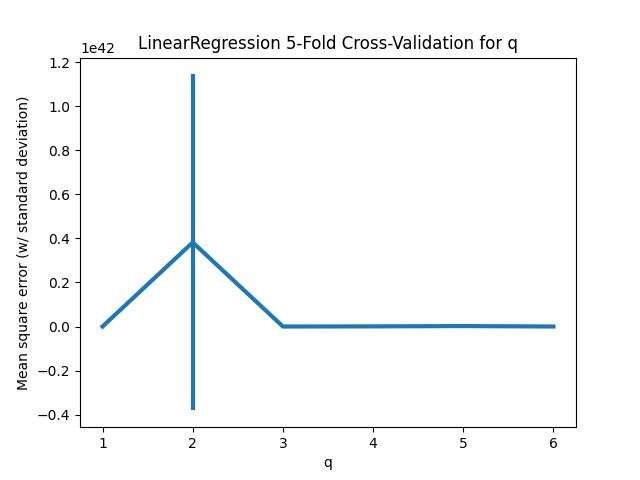
\includegraphics[width=\linewidth]{../graphs/stasis_webifier_linreg_polyfeatures_crossval.png}
				\captionof{figure}{Abyssal Stasis Webifier}
			\end{minipage}%
			\begin{minipage}{0.3\linewidth}
				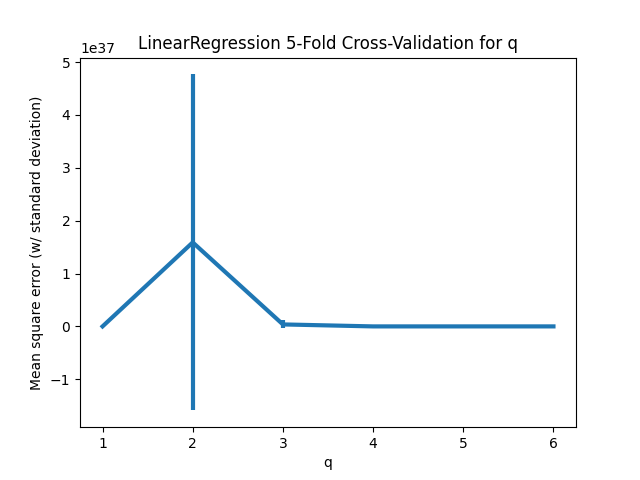
\includegraphics[width=\linewidth]{../graphs/shield_booster_linreg_polyfeatures_crossval.png}
				\captionof{figure}{X-Large Abyssal Shield Booster}
			\end{minipage}
		
			\begin{minipage}{0.3\linewidth}
				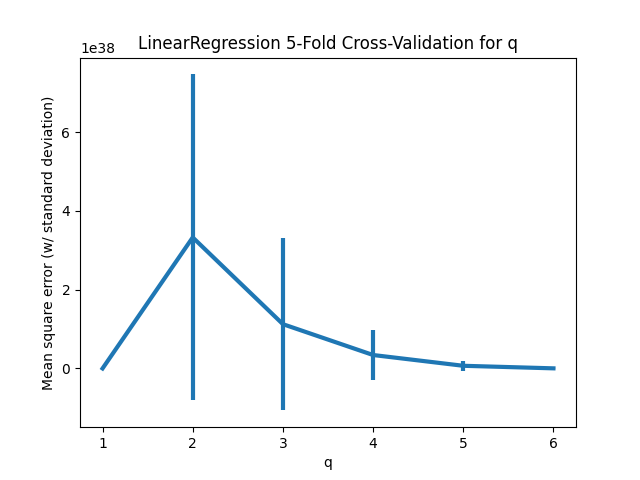
\includegraphics[width=\linewidth]{../graphs/afterburner_linreg_polyfeatures_crossval.png}
				\captionof{figure}{1MN Abyssal Afterburner}
			\end{minipage}%
			\begin{minipage}{0.3\linewidth}
				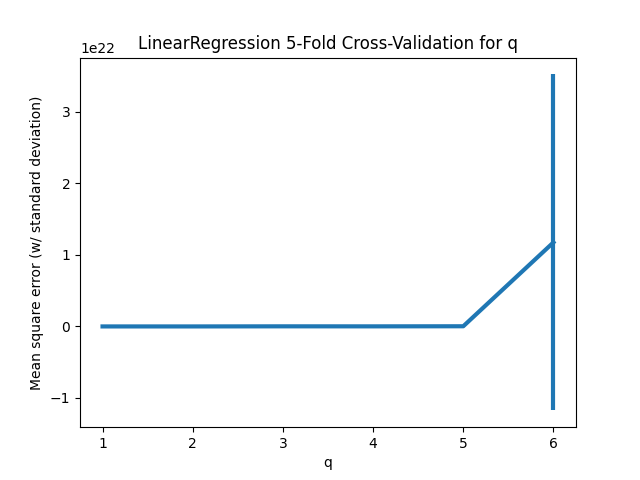
\includegraphics[width=\linewidth]{../graphs/entropic_radiation_sink_linreg_polyfeatures_crossval.png}
				\captionof{figure}{Abyssal Entropic Radiation Sink}
			\end{minipage}
		
	\subsection{Ridge Regression}		
		\begin{tabular}{|c|c|c|c|c|}
			\hline
			& Abyssal Entropic Radiation Sink & Abyssal Stasis Webifier & X-Large Abyssal Shield Booster & 1MN Abyssal Afterburner\\
			\hline
			$\alpha$ & 0.1 & 0.01 & 0.0001 & 0.01\\
			\hline
		\end{tabular}
	
		\begin{minipage}{0.29\linewidth}
			The Abyssal Entropic Radiation Sink had the largest value for $\alpha$, which suggests that Ridge Regression works best for this item when the magnitude of the parameters are kept small. X-Large Abyssal Shield Booster had the smallest value of $\alpha$, which suggests that it needs large parameter magnitudes to more accurately correlate its attributes to its price. The other two items' values of $\alpha$ fall in between, suggesting that their prices can best be predicted when the magnitude of the parameters is neither extremely large nor extremely small. The plots on the right show the MSE and standard deviation against $\alpha$ for each item to justify our choices. We typically chose the $\alpha$ with the smallest MSE, but for X-Large Abyssal Shield Booster that $\alpha$ had a much larger standard deviation, which led to our choice of 0.0001 over 0.1 as the difference between the MSEs was far smaller than the difference between the standard deviations.
		\end{minipage}\qquad%
		\begin{minipage}{0.9\linewidth}
			\begin{minipage}{0.35\linewidth}
				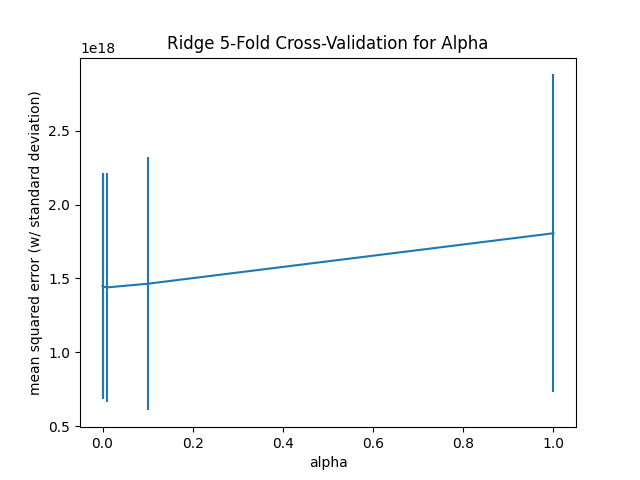
\includegraphics[width=\linewidth]{../graphs/stasis_webifier_ridge_alpha_crossval.png}
				\captionof{figure}{Abyssal Stasis Webifier}
			\end{minipage}%
			\begin{minipage}{0.35\linewidth}
				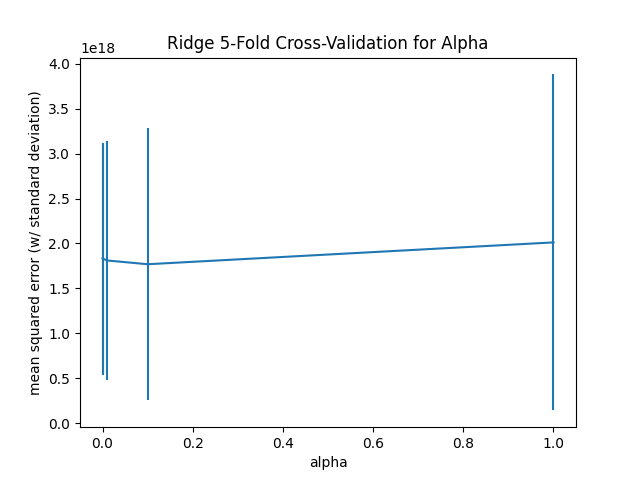
\includegraphics[width=\linewidth]{../graphs/shield_booster_ridge_alpha_crossval.png}
				\captionof{figure}{X-Large Abyssal Shield Booster}
			\end{minipage}
			
			\begin{minipage}{0.35\linewidth}
				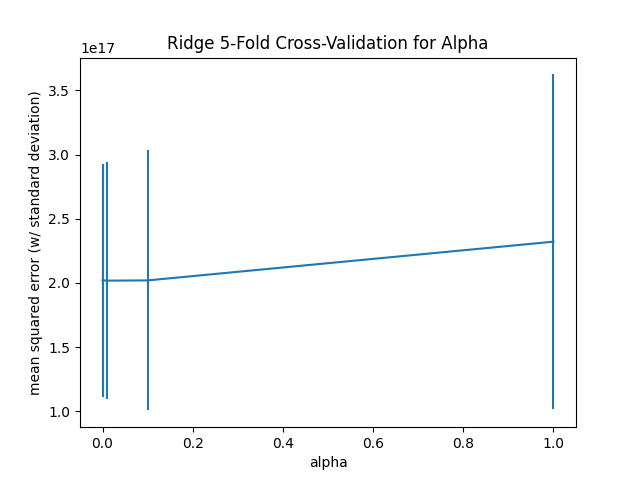
\includegraphics[width=\linewidth]{../graphs/afterburner_ridge_alpha_crossval.png}
				\captionof{figure}{1MN Abyssal Afterburner}
			\end{minipage}%
			\begin{minipage}{0.35\linewidth}
				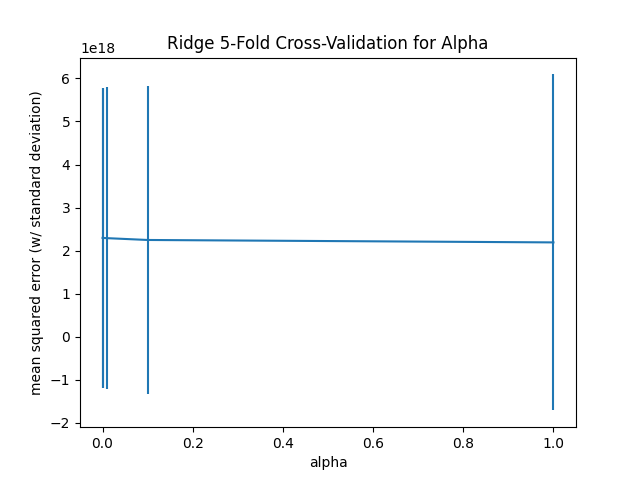
\includegraphics[width=\linewidth]{../graphs/entropic_radiation_sink_ridge_alpha_crossval.png}
				\captionof{figure}{Abyssal Entropic Radiation Sink}
			\end{minipage}
		\end{minipage}
	\subsection{Lasso Regression}
		\begin{tabular}{|c|c|c|c|c|}
			\hline
			& Abyssal Entropic Radiation Sink & Abyssal Stasis Webifier & X-Large Abyssal Shield Booster & 1MN Abyssal Afterburner\\
			\hline
			$\alpha$ & 0.0001 & 0.0001 & 0.0001 & 0.0001\\
			\hline
		\end{tabular}
		
		\begin{minipage}[t]{0.3\linewidth}
		The value of $\alpha$ for all of the items was the smallest chosen, which suggests that in order for lasso regression to be useful it needs the capacity to choose parameters with large magnitudes. It should be noted, however, that the average MSE and standard deviation for all of the values of $\alpha$ tested were very similar, as can be seen from the plots on the right, which also suggests that the value of $\alpha$ is not overly important when using lasso regression for the datasets tested.
		\end{minipage}\qquad%
		\begin{minipage}[t]{0.8\linewidth}
			\begin{minipage}{0.35\linewidth}
				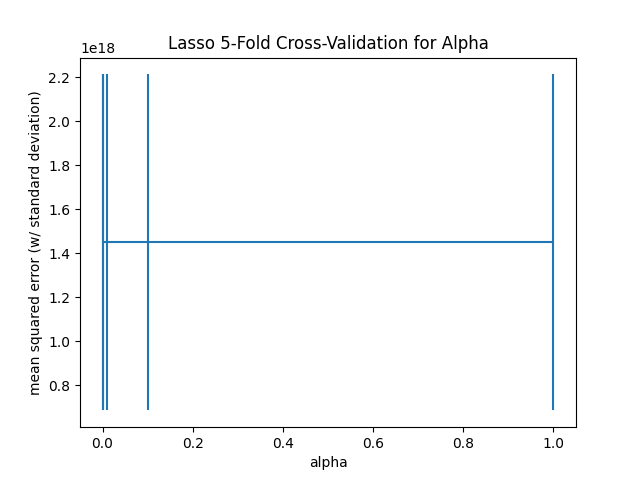
\includegraphics[width=\linewidth]{../graphs/stasis_webifier_lasso_alpha_crossval.png}
				\captionof{figure}{Abyssal Stasis Webifier}
			\end{minipage}\quad%
			\begin{minipage}{0.35\linewidth}
				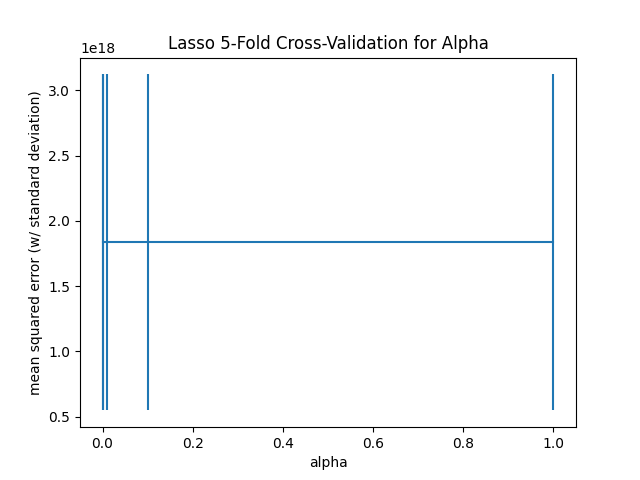
\includegraphics[width=\linewidth]{../graphs/shield_booster_lasso_alpha_crossval.png}
				\captionof{figure}{X-Large Abyssal Shield Booster}
			\end{minipage}
			
			\begin{minipage}{0.35\linewidth}
				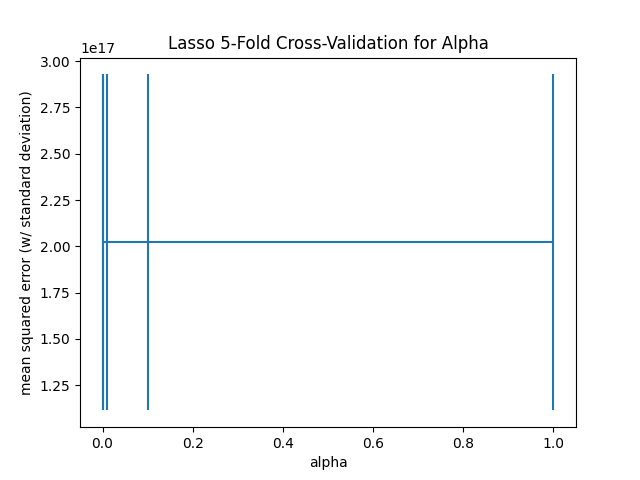
\includegraphics[width=\linewidth]{../graphs/afterburner_lasso_alpha_crossval.png}
				\captionof{figure}{1MN Abyssal Afterburner}
			\end{minipage}\quad%
			\begin{minipage}{0.35\linewidth}
				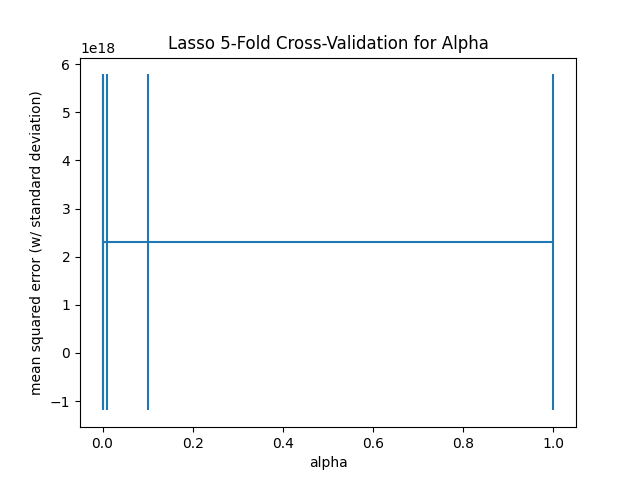
\includegraphics[width=\linewidth]{../graphs/entropic_radiation_sink_lasso_alpha_crossval.png}
				\captionof{figure}{Abyssal Entropic Radiation Sink}
			\end{minipage}
		\end{minipage}
	
	\subsection{Comparison}
		The table below shows the MSE for each item for the baseline model along with linear, ridge and lasso regression models using the hyperparameters chosen from cross-validation. 
		
		\medskip
		
		\begin{tabular}{|c|c|c|c|c|}
			\hline
			& Abyssal Entropic & Abyssal & X-Large Abyssal & 1MN Abyssal\\
			& Radiation Sink & Stasis Webifier & Shield Booster & Afterburner\\
			\hline
			Baseline MSE & $2.42335*10^{18}$ & $2.90456*10^{18}$ & $2.57651*10^{18}$ & $2.93333*10^{17}$\\
			Linear Reg. MSE & $2.29678*10^{18}$ & $1.44899*10^{18}$ & $1.83472*10^{18}$ & $1.98570*10^{17}$\\
			Ridge Reg. MSE & $2.24848*10^{18}$ & $1.43914*10^{18}$ & $1.83434*10^{18}$ & $2.01829*10^{17}$\\
			Lasso Reg. MSE & $2.29678*10^{18}$ & $1.44901*10^{18}$ & $1.83472*10^{18}$ & $2.02116*10^{17}$\\
			\hline
		\end{tabular}
	
		\medskip
	
		Ridge regression had the lowest MSE for Abyssal Entropic Radiation Sink, Abyssal Stasis Webifier and X-Large Abyssal Shield Booster.
		
		This indicates that having an L2 penalty helps to coerce the values in $\theta$ to their optimal values. For 1MN Abyssal Afterburner Linear Regression was the most effective model. This suggests that adding penalties to the cost function for this dataset failed to cause it to learn more about the data.
		
		The values of the MSEs, even when taken in context with the values of the item prices, are large. Given the small datasets that were used, this is unsurprising. In order to generate more accurate predictions a larger dataset collected over a far longer period of time is necessary. With the current dataset size over-fitting is possible, which could lead to the large MSEs we see here. However as the baseline model is comprehensively beaten for all items, this suggests that regression is a promising tool for price prediction and that further work with more data could yield useful results.
		
\section{Summary}
	The aim of the project was to create a model that predicted the selling price of a mutated module based on its statistics. Based on the experiments we discovered that polynomial regression with degree 1 produced predictions with the lowest average MSE, confirming the linear contribution of the features to the modules predicted selling price. The value of $\alpha$ for Lasso regression didn’t make a massive difference in terms of accuracy when applied to our project dataset. For all the mutated models tested we got similar values for the MSEs and Standard Deviation. For Ridge Regression there was more of a range when it came to optimal values for $\alpha$. Large values for $\alpha$ were better suited when the magnitude of parameters were small and smaller values for $\alpha$ were better suited when the magnitude of parameters were large. 
	
	To further improve on our final models it would be ideal to collect a larger dataset over a longer period of time to better understand trends and relationships between the model features and the output. This would allow us to build more accurate models that are not as prone to over/underfitting as discussed in the report.

\section{Appendix: Contributions}
	\textbf{Abraham Ayooluwa Odukoya:}\\
	Wrote the code for evaluating linear, ridge and lasso regression and performing cross validation to find $\alpha$ for ridge and lasso regression. Ran the cross-validation experiments to choose the hyperparameters and to evaluate the final models. Wrote the linear regression, ridge regression and lasso regression parts of the Methods section and contributed to the experiments and results sections.
	
	\textbf{Sharon Olorunniwo:}\\
	Wrote the code for evaluating our model with polynomial features and performing cross validation to find the optimal q (number of degrees) for the polynomial regression model. Wrote the introduction, polynomial features section of the methods section, contributed to the experiments and results section and wrote the Summary.
	
	\textbf{Jack Harley:}\\
	Wrote the code for scraping, storing and accessing the data from the EVE servers, set up and administered the cloud server for the automated scheduled scraping. Wrote the introduction to the report and the dataset/features section. Helped plan the various machine learning models. Converted the draft report into LaTeX and produced the final edit for submission.
		
\end{document}
